\chapter{实验结果与分析}
本章将对实验进行检验并对比分析:将统计各个类的AP值并做出PR曲线;预测效果展示,并展现其中效果不佳的结果;探究实验泛化性能力。
\section{实验平台}{
	基本环境:
	\begin{enumerate}
		\item 操作系统: CentOS Linux release 7.1
		\item 显卡: GTX1080
		\item CUDA版本: 8.0
		\item 实验框架: Darknet
		\item 数据集: KITTI
	\end{enumerate}

	YOLO训练参数:
	\begin{enumerate}
		\item batch size: 64
		\item width: 416
		\item height: 416
		\item channels: 3
		\item momentum: 0.9
		\item decay: 0.0005
		\item learing rate: 0.001
		\item max batches: 50000
	\end{enumerate}

	tiny-YOLO训练参数:
	\begin{enumerate}
		\item batch size: 64
		\item width: 416
		\item height: 416
		\item channels: 3
		\item momentum: 0.9
		\item decay: 0.0005
		\item learing rate: 0.001
		\item max batches: 50000
	\end{enumerate}

	如图\ref{},展现了两个模型的训练过程。
}

\newpage

\section{结果对比}{
	\subsection{AP比较}
	\begin{table}  
	\caption{各模型各类AP和FPS结果对比}  
	\begin{tabular}{l|p{2cm}p{2cm}p{2cm}p{2cm}}  
	\hline  
	             & Pedestrian & Car      & Cyclist  & FPS \\  
	\hline  
	Faster R-CNN & 65.91 \%   & 79.11 \% & 62.81 \% & 0.5 \\  
	YOLO         & 51.44 \%   & 68.05 \% & 50.97 \% & 45  \\
	tiny-YOLO    & 26.67 \%   & 50.75 \% & 25.04 \% & 120  \\
	\hline
	\end{tabular}
	\label{AP}
	\end{table} 
	我们首先对比本项目各个模型对于各个类的AP值以及FPS比较,如表\ref{AP}。其中Faster R-CNN的数据参考自\ref{}。

	通过图表,我们可以发现虽然tiny-YOLO有120fps,而yolo只有45fps,比YOLO的速度快上2-3倍,但是性能远不如YOLO。从速度上来看,YOLO能达到每秒45帧的速度,已经基本可以满足实时行人检测的需求,tiny-YOLO甚至然能够达到每秒120帧的速度,两个模型均能满足实时行人检测的要求。从性能上来看,不管是哪个类的AP值,YOLO都全面领先于tiny-YOLO,尤其是在行人和自行车的检测上,而YOLO不仅在行人和自行车上能分别达51.44AP和50.97AP,在车辆检测上更是能达到68.05AP,效果较好。而反观tiny-YOLO,它在车辆检测上只有50.75AP,而在行人检测和自行车检测上更是仅有26.67AP和25.04AP

	从整体上看,模型对车辆的检测明显高于对行人和自行车的检测,这是由于KITTI数据集中车辆数据较多造成的。而模型的整体表现也部分受限于训练数据过少。

	对比Faster R-CNN,Faster R-CNN仅有0.5fps,无法满足实时行人检测的要求,不管是YOLO还是tiny-YOLO,在速度上都明显比Faster R-CNN要快上很多。并且Faster R-CNN在行人、车辆、自行车上的检测分别有65.91AP、79.11AP、62.81AP,YOLO在这三项上的损失并没有想象上的那么大。可见YOLO仅牺牲了部分的精度确在检测速度上提高了很多。

	总的来说,YOLO在AP上的表现达到预期效果,而tiny-YOLO虽然速度很快,但是效率上损失过多。

	\subsection{PR曲线比较}
	\begin{figure}[htbp]
	\centering
	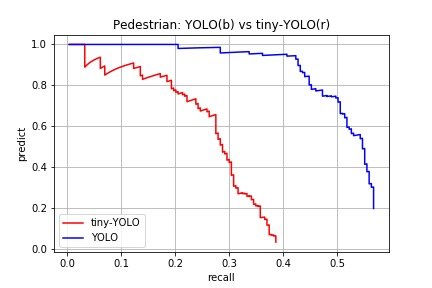
\includegraphics[width=5in]{images/pedestrianPR.png}
	\caption{行人检测比较}
	\label{pedestrianPR}
	\end{figure}
	\begin{figure}[htbp]
	\centering
	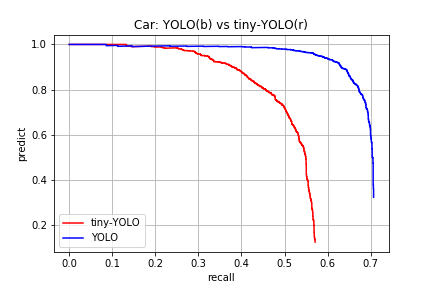
\includegraphics[width=5in]{images/carPR.png}
	\caption{车辆检测比较}
	\label{carPR}
	\end{figure}
	\begin{figure}[htbp]
	\centering
	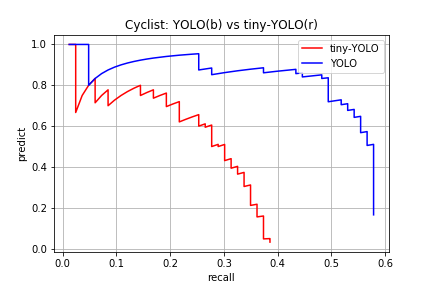
\includegraphics[width=5in]{images/cyclistPR.png}
	\caption{自行车检测比较}
	\label{cyclistPR}
	\end{figure}
	我们分别对各个模型各个类做出PR曲线并进行比较,结果如图\ref{pedestrianPR,carPR,cyclistPR}。

	从图\ref{pedestrianPR}中可以看出,对于行人的检测上,YOLO模型明显好于tiny-YOLO的模型,在召回率0.4的时候,tiny-YOLO的准确率已经接近0,而YOLO的准确率还是接近1。

	从图\ref{carPR}中可以看出,对于车辆的检测,两个模型都有很好的表现,PR曲线都很飘。tiny-YOLO大概在召回率大于0.45后准确率开始快速下降,而YOLO则在召回率大于0.6后准确率快速下降。

	从图\ref{cyclistPR}中可以看出,对于自行车的检测,YOLO模型也明显好于tiny-YOLO模型。tiny-YOLO下降速度比较稳定,而YOLO在召回率大于0.5后准确率开始快速下降。
}

\section{预测效果}{
	\subsection{效果展示}

	\subsection{错误结果分析}
}

\section{泛化性}{
	本项目讨论实时行人检测的可行性,针对日常生活驾驶、极端天气、夜晚等各种情形进行实验。
}

\section{本章小结}


